\section{Simulation}
\subsection{Monte Carlo Simulation}
Monte Carlo Simulation ist eine numerische Methode für statistische Simulation, die Sequenzen von Zufallszahlen benutzt, um die Simulation durchzuführen.

\textbf{Eigenschaften:}
\begin{compactitem}
	\item Monte Carlo Simulation ist ein kräftiges Instrument, um komplexe statistische Analysen durchzuführen und Wahrscheinlichkeiten und Verteilungen zu schätzen.
	\item Es verlangt ein Systemmodell (quantitative Systembeschreibung).
	\item Es werden (virtuelle) Experimente mit dem System ausgeführt, um Schlussfolgerungen bzgl. deren Verhalten zu ziehen.
\end{compactitem}

\begin{example}
	Berechne den Wert von $\pi$
	\begin{multicols}{5}
		Fläche Rechteck: $(2r)^2$ \\
		Fläche Kreis: $\pi r^2$ \\
		$\frac{\text{Fläche Rechteck}}{\text{Fläche Kreis}}$: $\frac{4}{\pi}$ \\
		$\pi$: $4 * \frac{\text{Fläche Kreis}}{\text{Fläche Rechteck}}$ \\
		$\pi$: $4 * \frac{\text{Punkte im Kreis}}{\text{Punkte im Rechteck}}$	
	\end{multicols}
	\begin{minipage}[h]{0.825\textwidth}
		\begin{lstlisting}[mathescape=true, tabsize=2]
N Punkte $X_i$ = -1 + 2$A_i$ und
N Punkte $Y_i$ = -1 + 2$B_i$ mit A, B Sequenzen von unabhaengigen Zufallszahlen
K = 0
for i = 1 : N
	if ($X_i^2$ + $Y_i^2$ < 1)
		K = K + 1
	end
end
$\pi$ = 4 * K / N
		\end{lstlisting}
	\end{minipage}
	\begin{minipage}[h]{0.175\textwidth}
		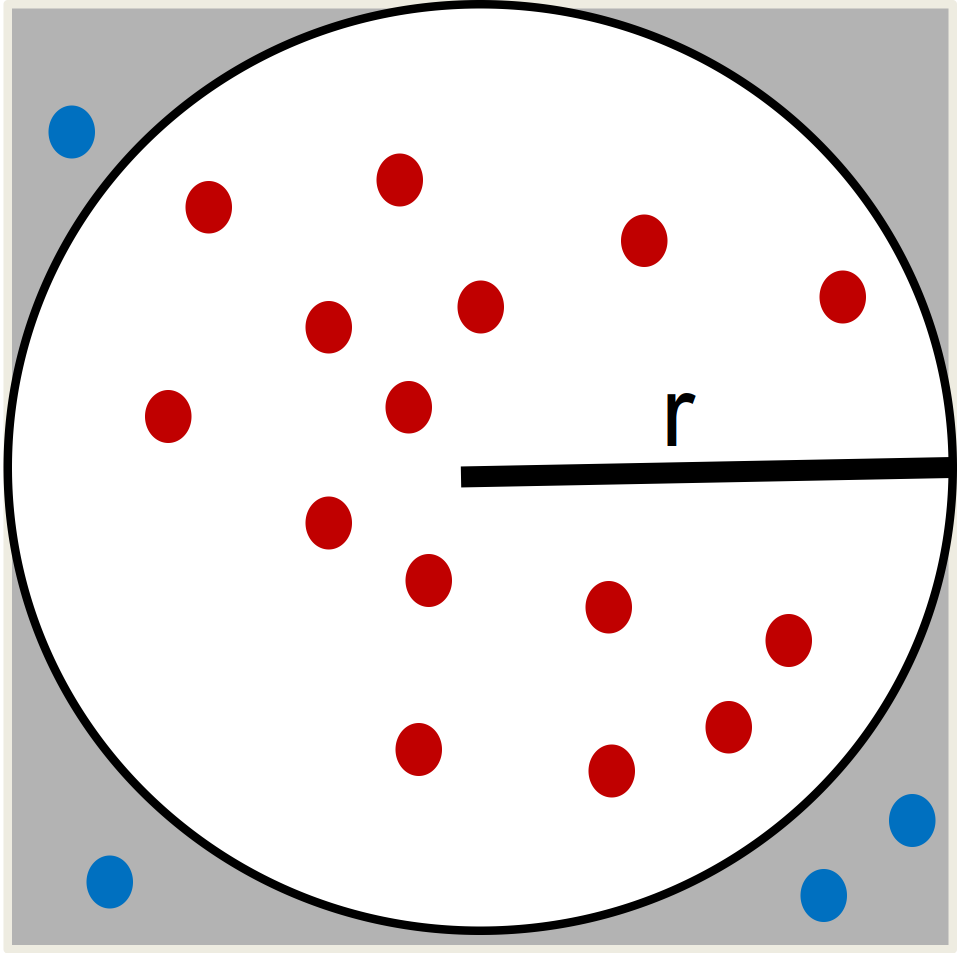
\includegraphics[width=1\textwidth]{pictures/montecarlopi}
	\end{minipage}
\end{example}

\subsection{Diskrete Ereignissimulation}
\subsubsection{Warteschlangentheorie}
Die Warteschlangentheorie beschäftigt sich mit der mathematischen Analyse von Systemen, in denen Aufträge von Bedienungsstationen bearbeitet werden und gibt Antwort auf die Fragen nach den charakteristischen Grössen, wie der Stabilität des Wartesystems, der Anzahl Kunden im System, ihrer Wartezeit etc. Sie unterstützt unter anderem Führungsentscheidungen über den Personaleinsatz und den Abfertigungsprozess. Ihre Anwendung reicht von Telekommunikationssystemen, Verkehrssystemen über Logistik bis zu Fertigungssystemen.
\begin{example}\\
	\begin{tabular}{|l|l|l|}
		\hline
		\textbf{System} & \textbf{Bedienungsstation} & \textbf{Aufträge} \\ \hline
		Bank & Schalter & Kundenbesuche \\ \hline
		Spital & Ärzte, Pflegende, Betten & Patientinnen und Patienten \\ \hline
		Rechner & CPU, I/O-Geräte & Jobs \\ \hline
		Fertigung & Maschinen, Operateure & Bauteile \\ \hline
		Rettungsdienst & Rettungsfahrzeuge, Notfallärzte & Patientinnen und Patienten \\ \hline		
	\end{tabular}
\end{example}

\subsubsection{Hauptmerkmale}
\begin{compactitem}
	\item Anwesenheit stochastischer Prozesse
	\item Zeit(-ablauf) spielt eine wichtige Rolle.
	\item Wertveränderungen der Variablen werden verursacht durch Ereignisse und treten nur an diskreten Zeitpunkten auf.
\end{compactitem}

\begin{multicols}{2}
	\textbf{Vorteile:}
	\begin{compactitem}
		\item Kostengünstiges und sicheres Experimentierfeld
		\item Ermöglicht Analyse komplexer Systeme durch hohen Detaillierungsgrad
		\item Ermöglicht Animation und steigert somit Systemverständnis
	\end{compactitem}
	\textbf{Nachteile:}
	\begin{compactitem}
		\item Erfordert einen hohen initialen Zeitaufwand
		\item Bau eines Simulationsmodells ist relativ fehleranfällig
		\item Interpretation der Analysedaten ist anspruchsvoll
	\end{compactitem} \ \\
\end{multicols}

\subsubsection{M/M/1 Modell}
\begin{multicols}{3}
	\begin{compactitem}[$\bullet$]
		\item M-Elemente betreten Warteschlange
		\item M-Elemente sind in Warteschlange
		\item 1-Element verlässt Warteschlange
	\end{compactitem}
\end{multicols}
\begin{example}\\
	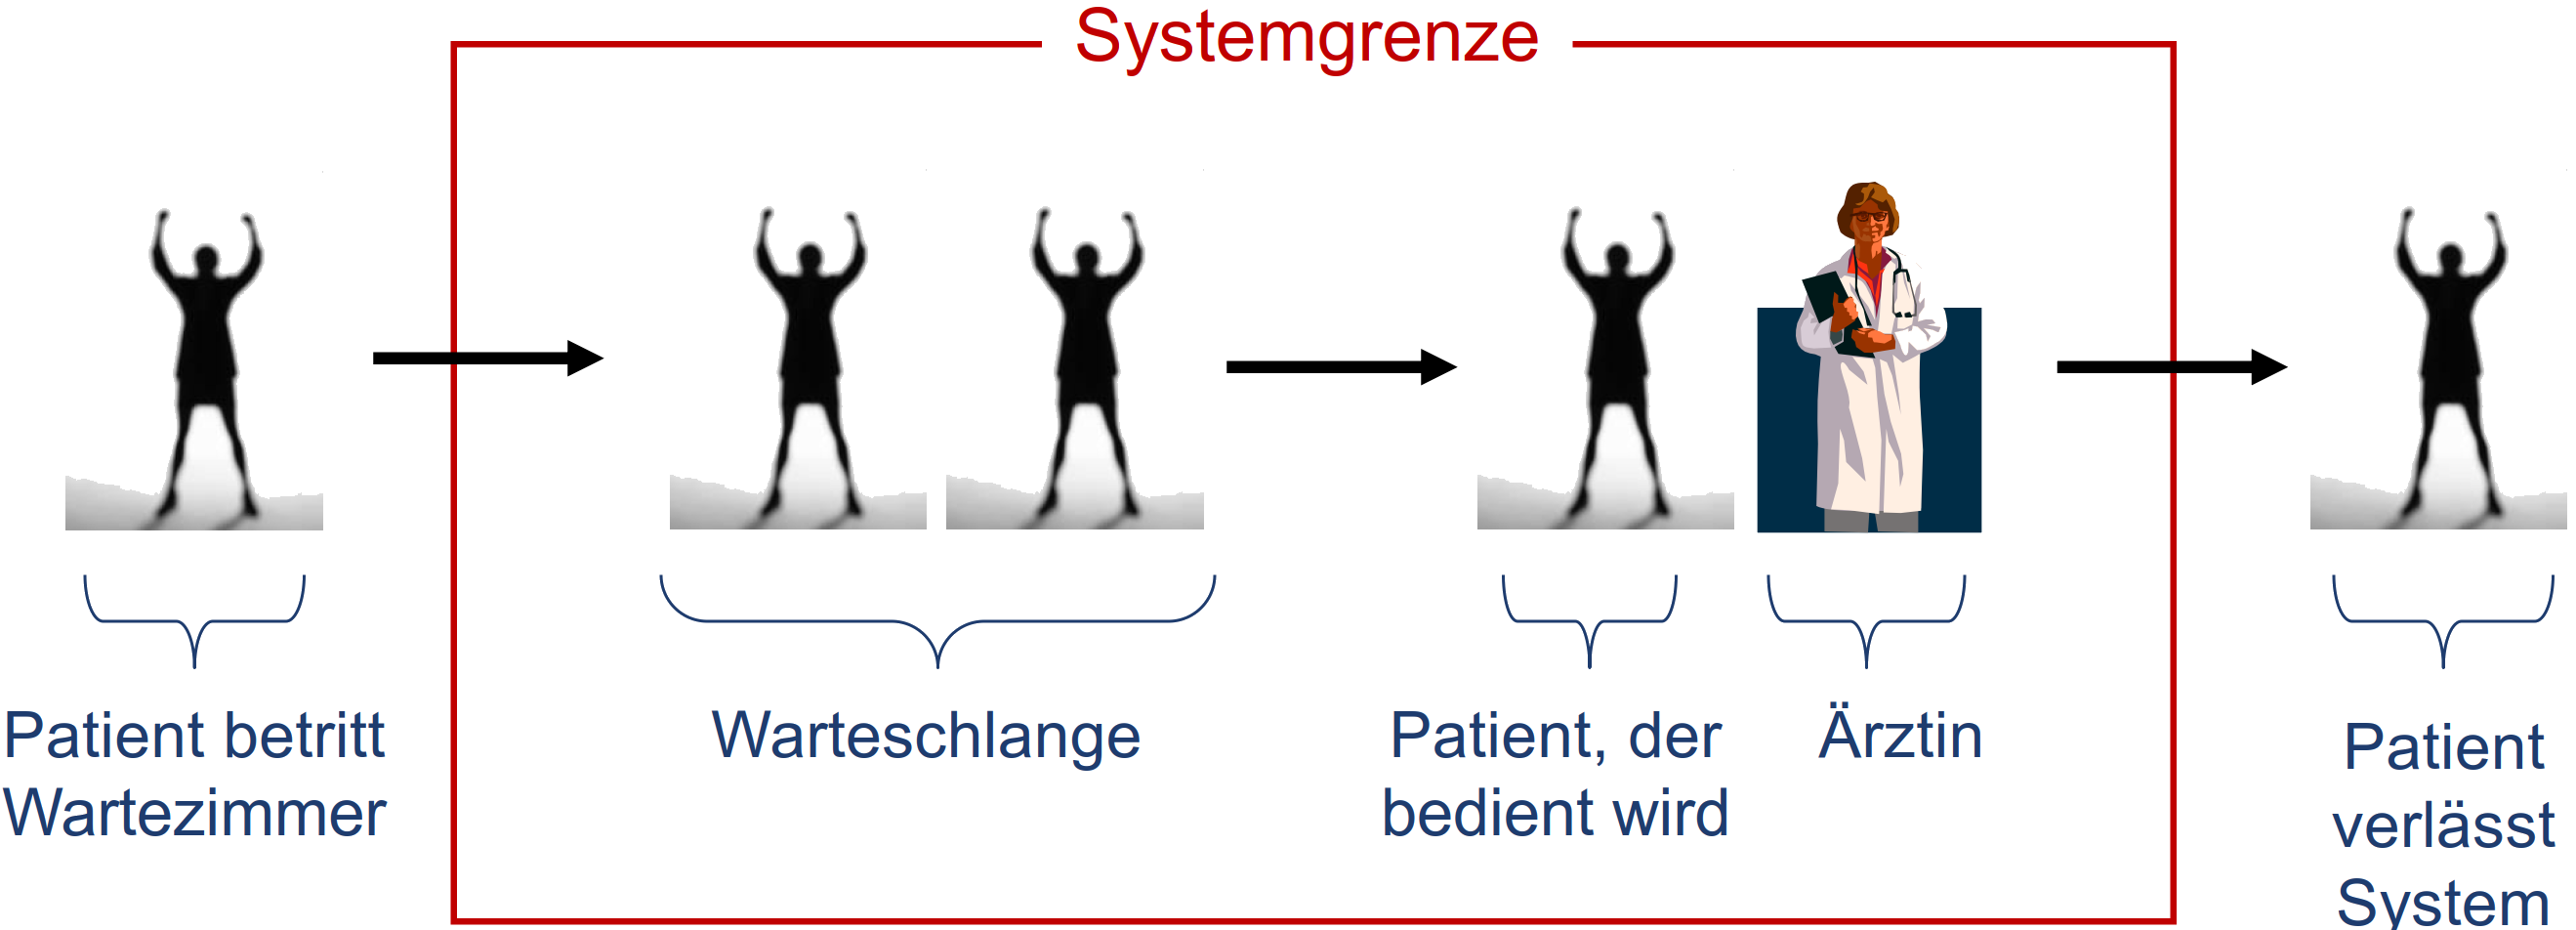
\includegraphics[width=0.7\textwidth]{pictures/mm1modell}
\end{example}
\todo{Folie 32 - Diagramme allenfalls noch einfügen}

\subsubsection{Kernelemente}
\textbf{Items:} Objekte, die durch das System fliessen (z.B. Patienten, Erstzteile, ...). Items haben meistens Attribute (Ankunftszeit, Bearbeitungsstartzeit, Prioritätsklasse, usw.). \\
\textbf{Systemzustand:} Der Zustand $Z(t)$ gibt eine vollständige Beschreibung des Systems am Zeitpunkt $t$. Der Systemzustand ist meistens ein (mehrdimensionaler) Vektor und dient u.a. der Berechnung der Zielgrössen. \\
\textbf{Simulationsuhr:} Die Simulationsuhr hält die virtuelle Zeit im Simulationsmodell fest. \\
\textbf{Ereignis:} Jedes Ereignis hat eine Wirkung, die zum Auftretenszeitpunkt ausgeübt wird. Die Wirkung besteht aus einer Änderung des Systemzustands und/oder einer Änderung der Future-Event-List. In der Zeit zwischen zwei nachfolgenden Ereignissen passiert im System nichts (der Systemzustand ändert sich nicht). Aus diesem Grund kann die Simulationsuhr von Ereignis zu Ereignis springen. \\
\textbf{Future Event List:} Dynamische Liste, die 0 oder mehr (Zeitpunkt-, Ereignis-) Paare enthält; Sie umfasst alle Ereignisse, die zum aktuellen Zeitpunkt bekannt sind. Während eines Simulationslaufs werden ständig neue Ereignisse hinzugefügt und verarbeitete Ereignisse gelöscht.

\subsubsection{Spezifikation eines DE Modells}
DE Modelle werden spezifiziert durch
\begin{compactenum}
	\item Flussdiagramme
	\item Ereignisdiagramme
\end{compactenum}
\todo{Nachführen}
\begin{example}[Beispiel für nachfolgende Kapitel 4.2xx]
	Wir betrachten eine Maschine, worauf genau ein Produkt hergestellt wird. Der Ankunftsprozess der Produktionsaufträge ist poissonverteilt mit dem Parameterwert $\lambda$. Bearbeitungszeiten sind exponentialverteilt mit dem Parameterwert $\mu$.\\
	Bei der Produktion können Fehler auftreten. Beim Maschinenausgang werden die Produkte visuell kontrolliert. Die Wahrscheinlichkeit eines Fehlers ist $\epsilon$. Misslungene Produktionsaufträge müssen wiederholt werden. \\
	\textbf{Items:} Produktionsaufträge mit Attributen: Ankunftszeit, Bearbeitungsstartzeit, Bearbeitungszeit, Anzahl Fehlversuche, etc. \\
	\textbf{Zustand:} $Z$ = (Anzahl) Produktionsaufträge im System \\
	\textbf{Ereignisse:} $e_1$ = Ankunft eines Produktionsauftrags; $e_2$ = Bearbeitung auf der Maschine abgeschlossen
\end{example}

\subsubsection{Flussdiagramm}
\textbf{Grundbausteine:}
\begin{multicols}{5}
	Quelle und Senke: \\ \\
	Fluss: \\ \\
	Weiche: \\ \\
	Warteschlange: \\ \\
	Aktivität oder Ressource:
\end{multicols}	
\begin{multicols}{5}
	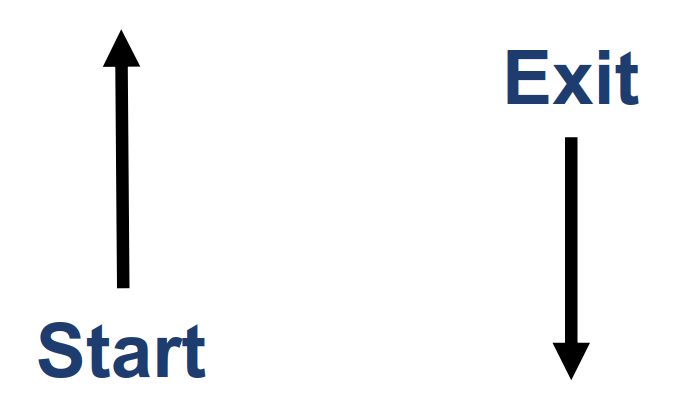
\includegraphics[width=0.15\textwidth]{pictures/fluss_quelle_senke}\\ \\
	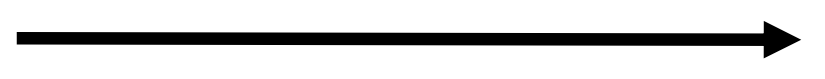
\includegraphics[width=0.15\textwidth]{pictures/fluss_fluss}\\
	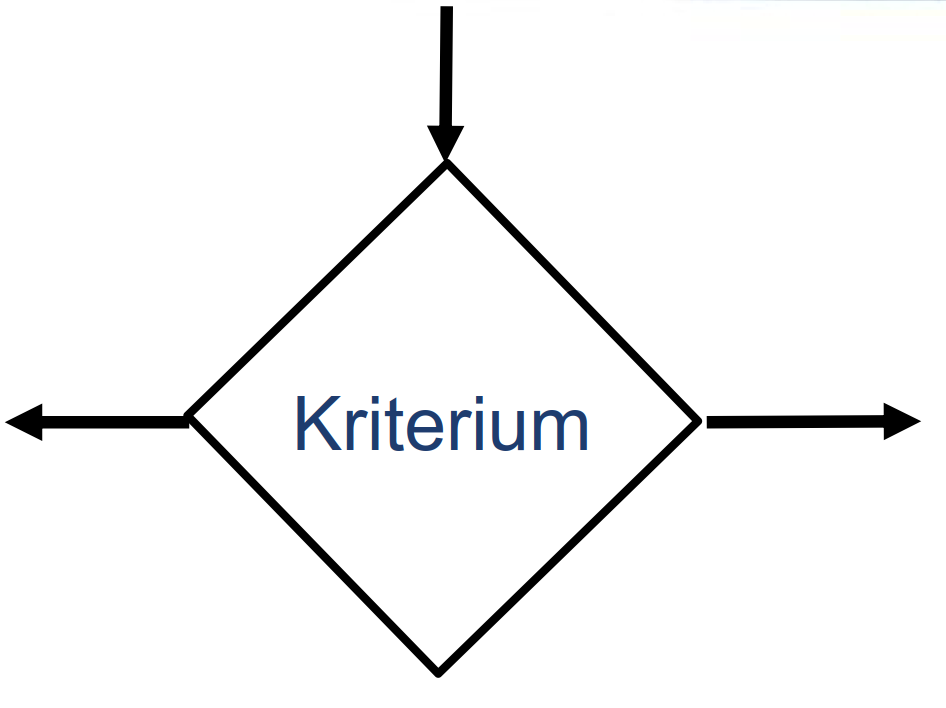
\includegraphics[width=0.15\textwidth]{pictures/fluss_weiche}\\ 
	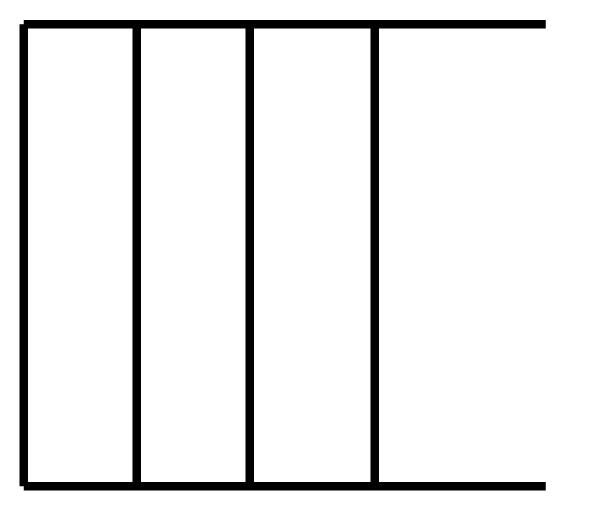
\includegraphics[width=0.1\textwidth]{pictures/fluss_warteschlange}\\ 
	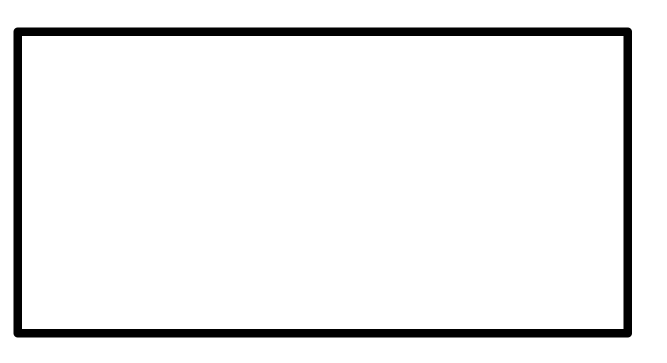
\includegraphics[width=0.15\textwidth]{pictures/fluss_aktivitaet}
\end{multicols}
\begin{multicols}{2}
	\begin{multicols}{2}
		Gabelung (konvergent):\\
		Gabelung (divergent):
	\end{multicols}
	Lager:
\end{multicols}
\begin{multicols}{2}
	\begin{multicols}{2}
		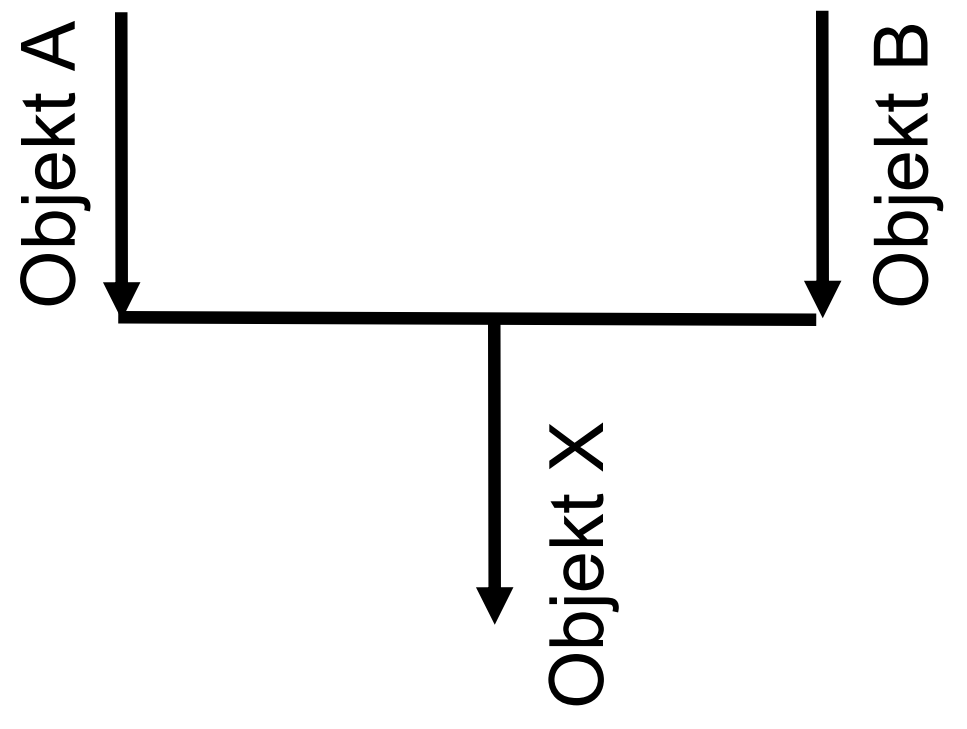
\includegraphics[width=0.2\textwidth]{pictures/fluss_gabelung1}\\ 
		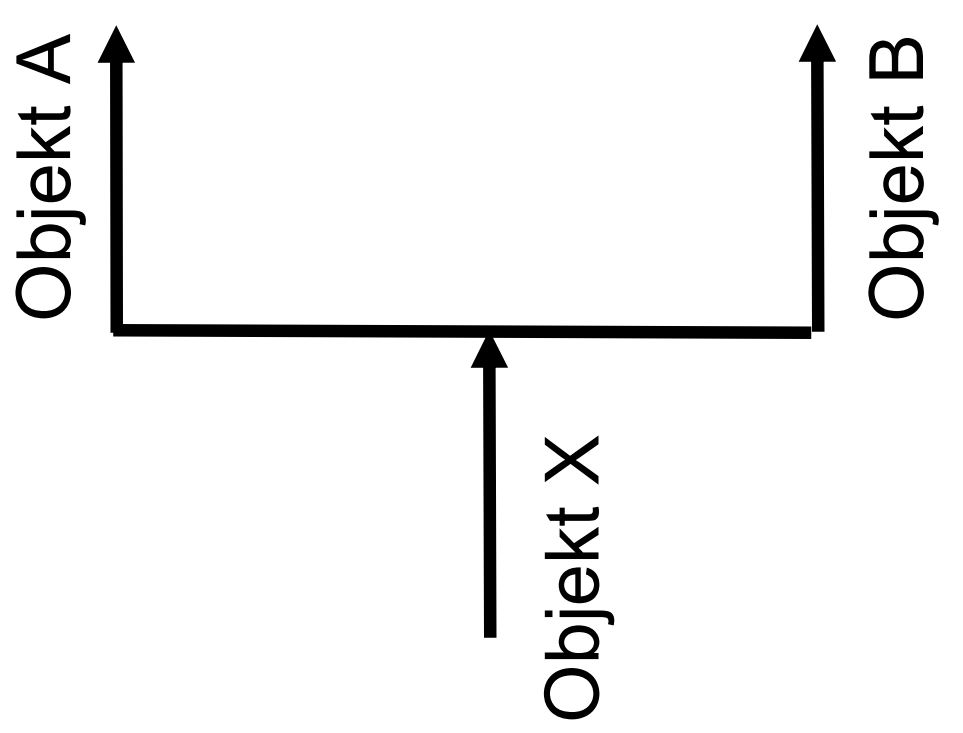
\includegraphics[width=0.2\textwidth]{pictures/fluss_gabelung2}
	\end{multicols}
	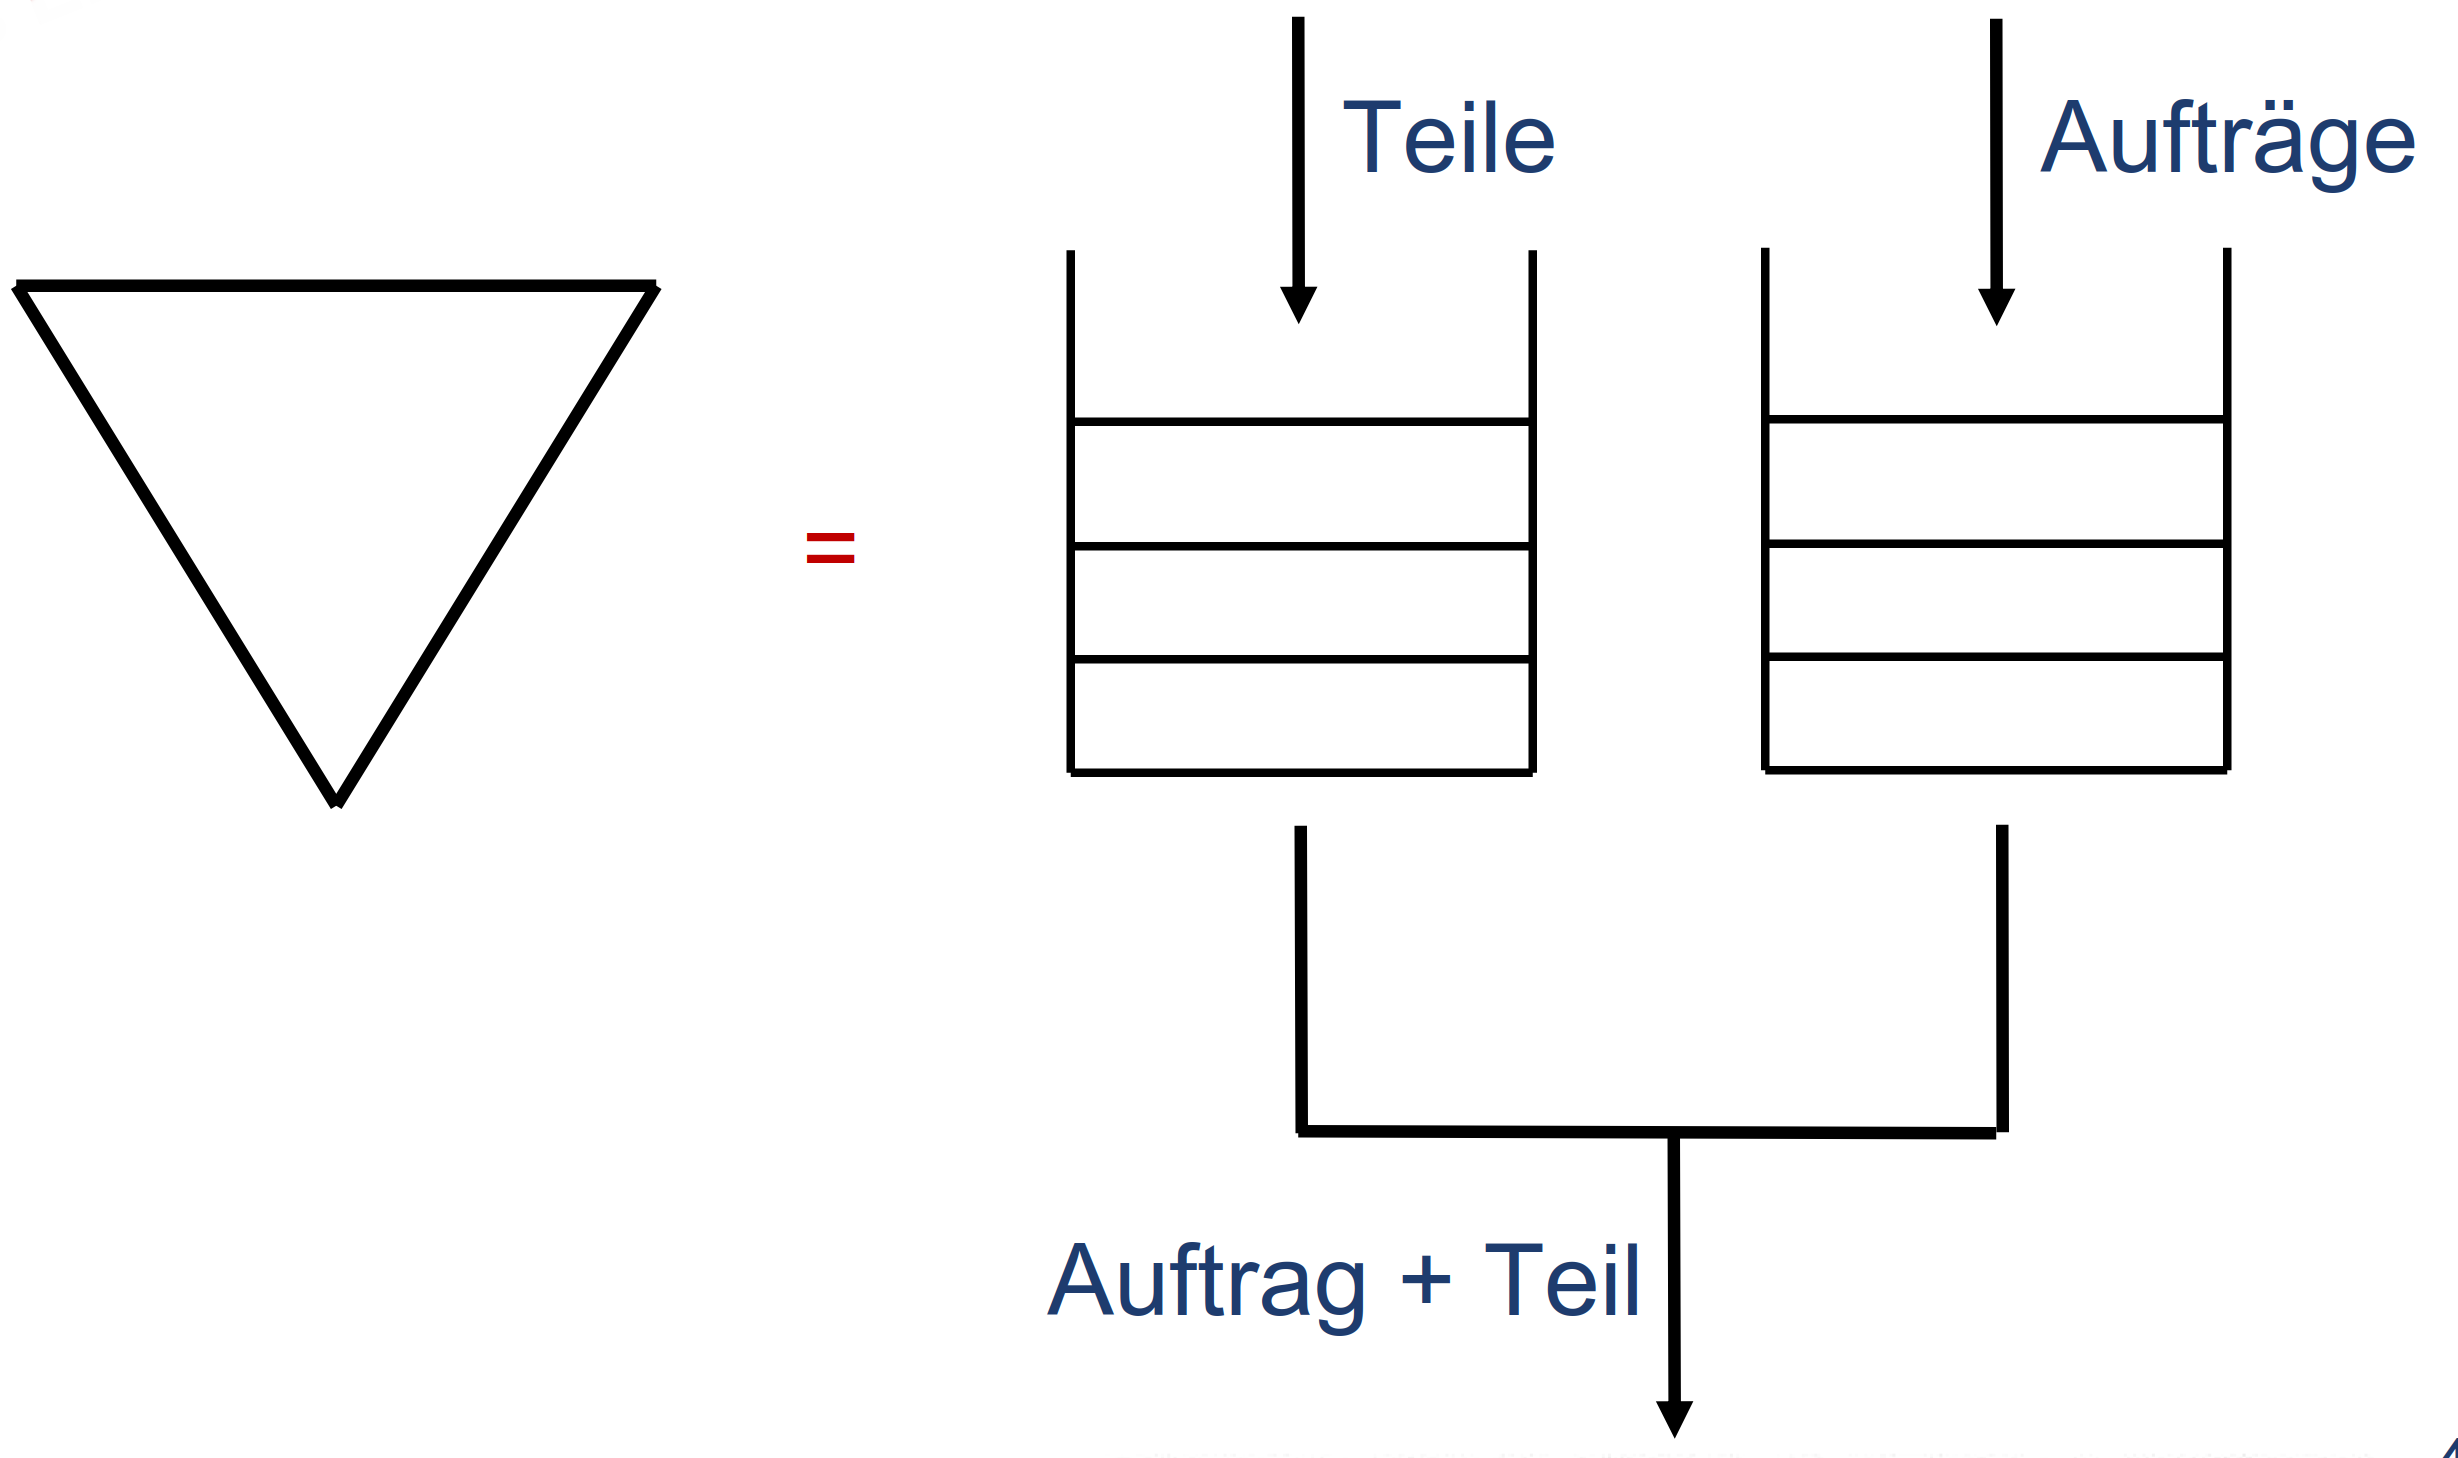
\includegraphics[width=0.45\textwidth]{pictures/fluss_lager}
\end{multicols}
\begin{example} \\
	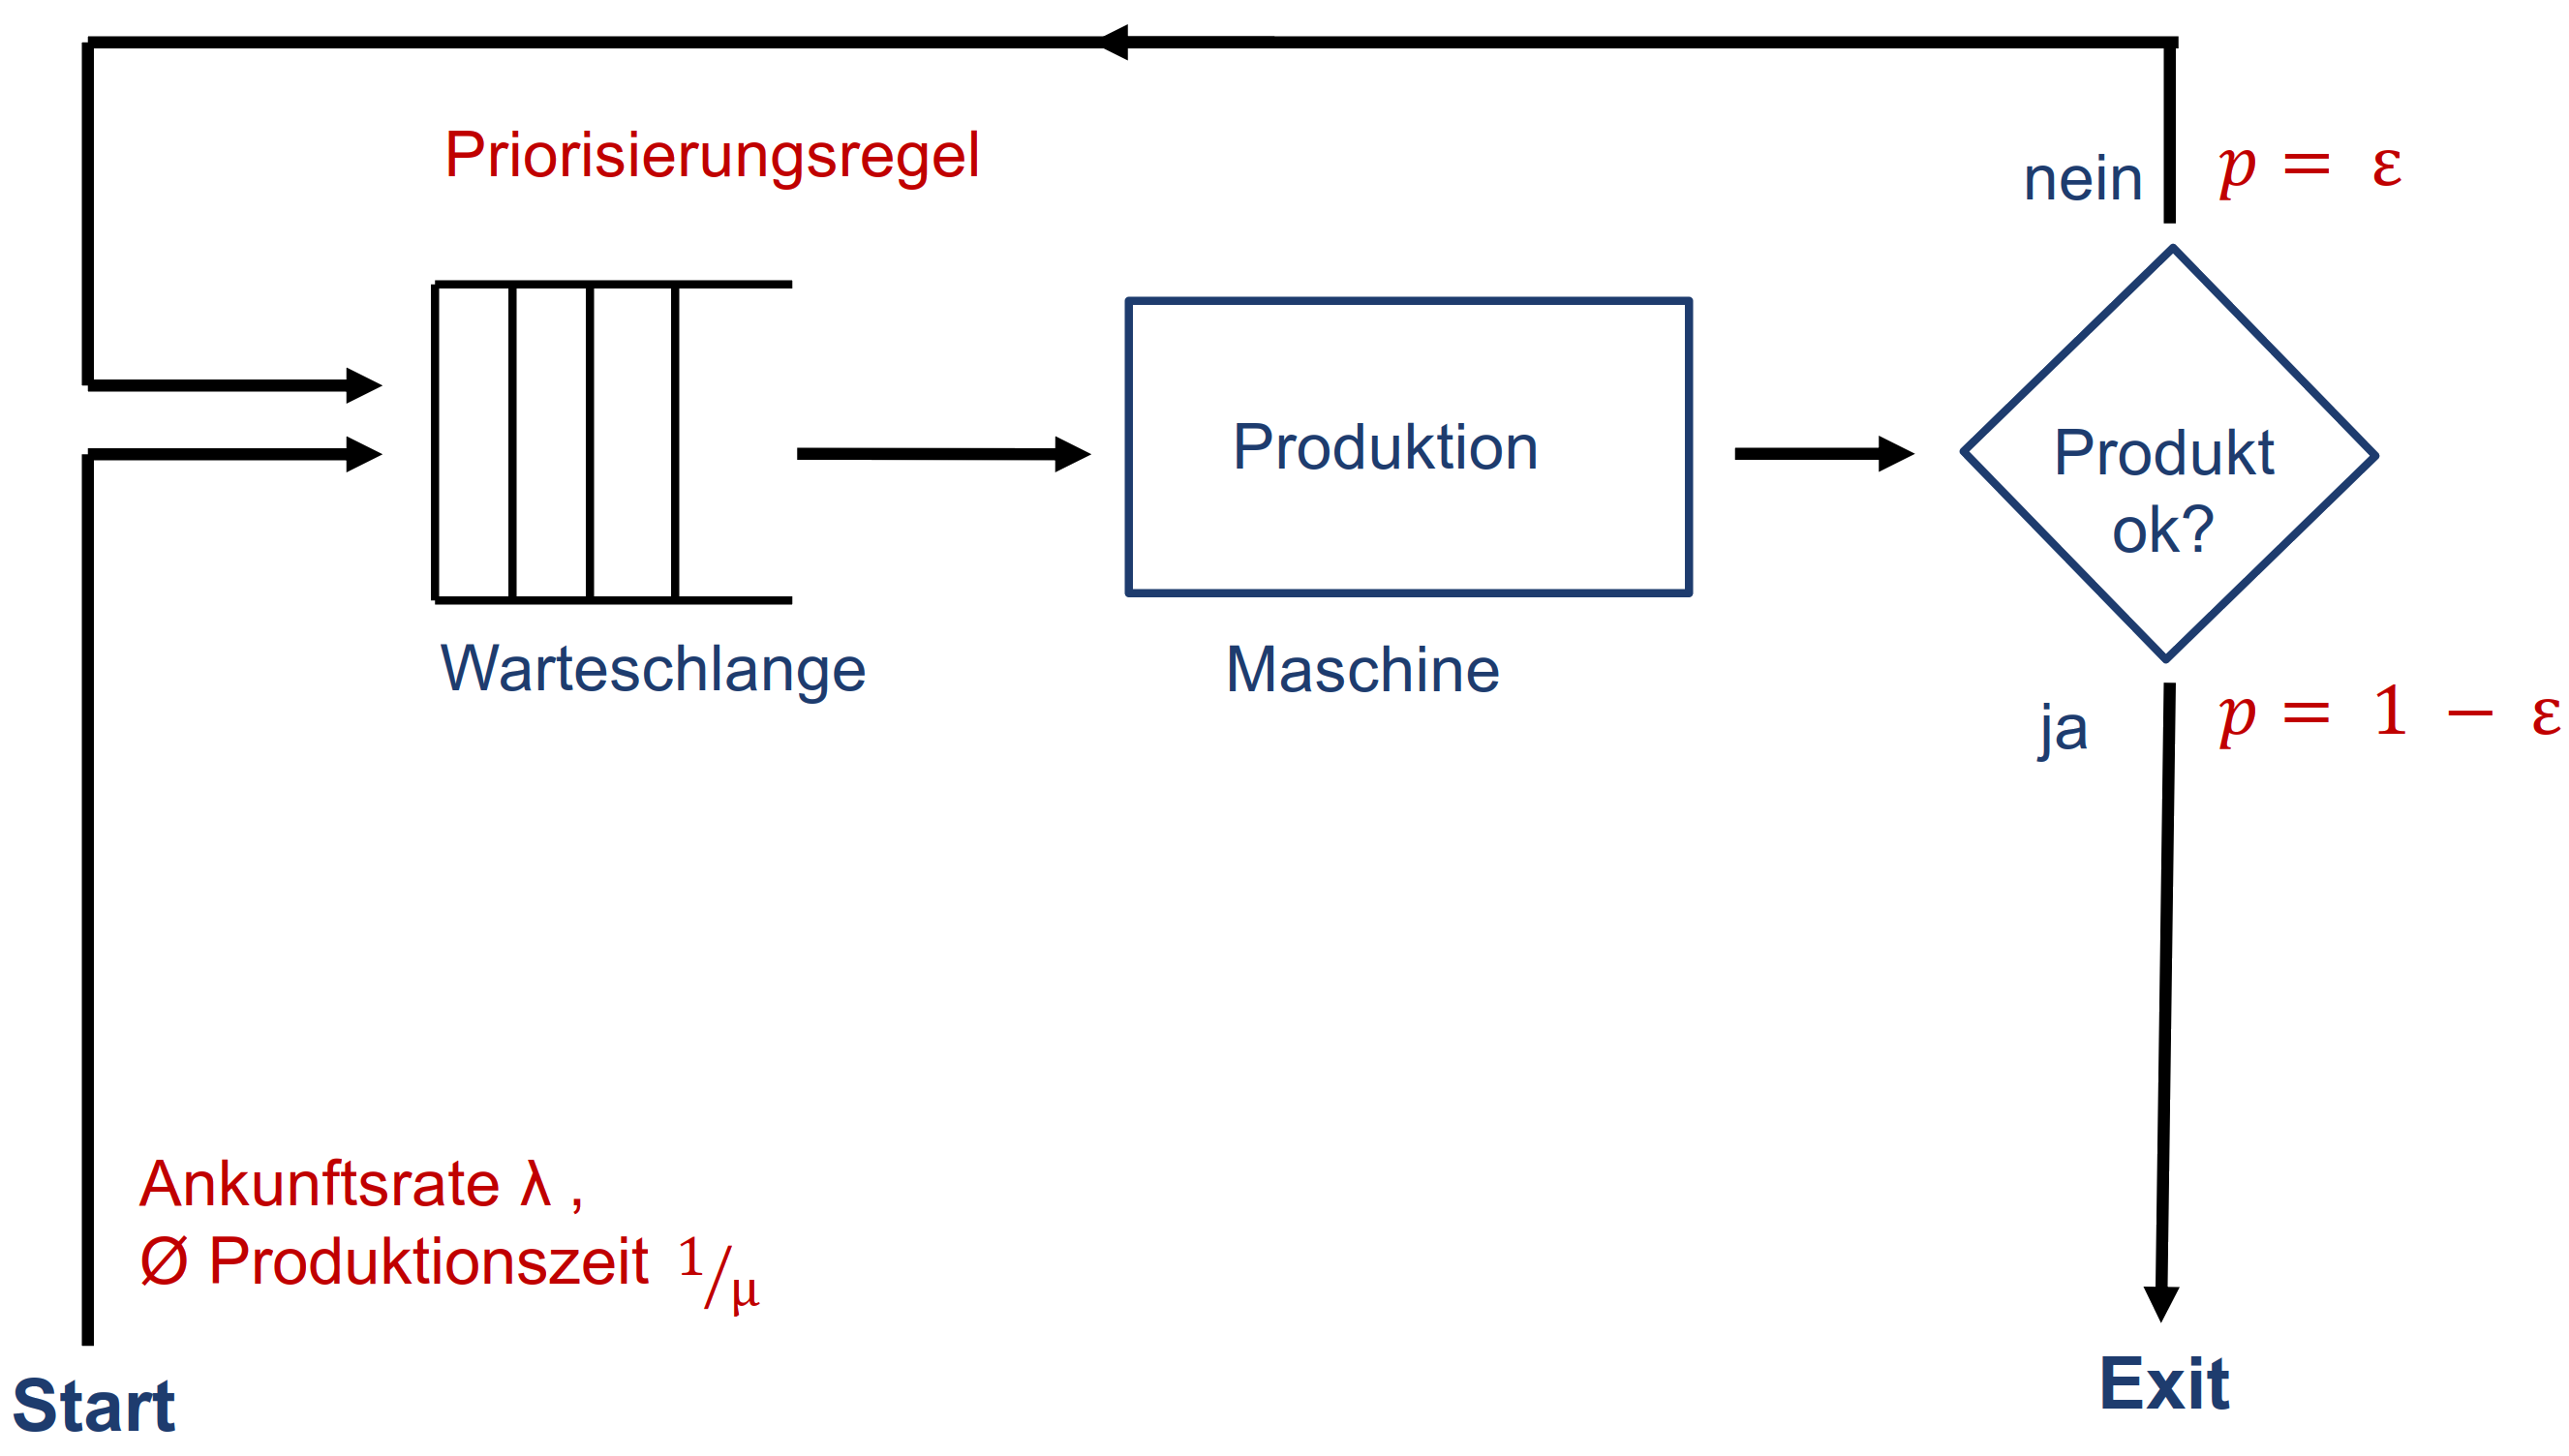
\includegraphics[width=0.45\textwidth]{pictures/flussdiagramm}
\end{example}

\subsubsection{Ereignisdiagramm}
\begin{example} \\
	\begin{multicols}{2}
		\textbf{Ereignisdiagramm $e_1$:} \\
		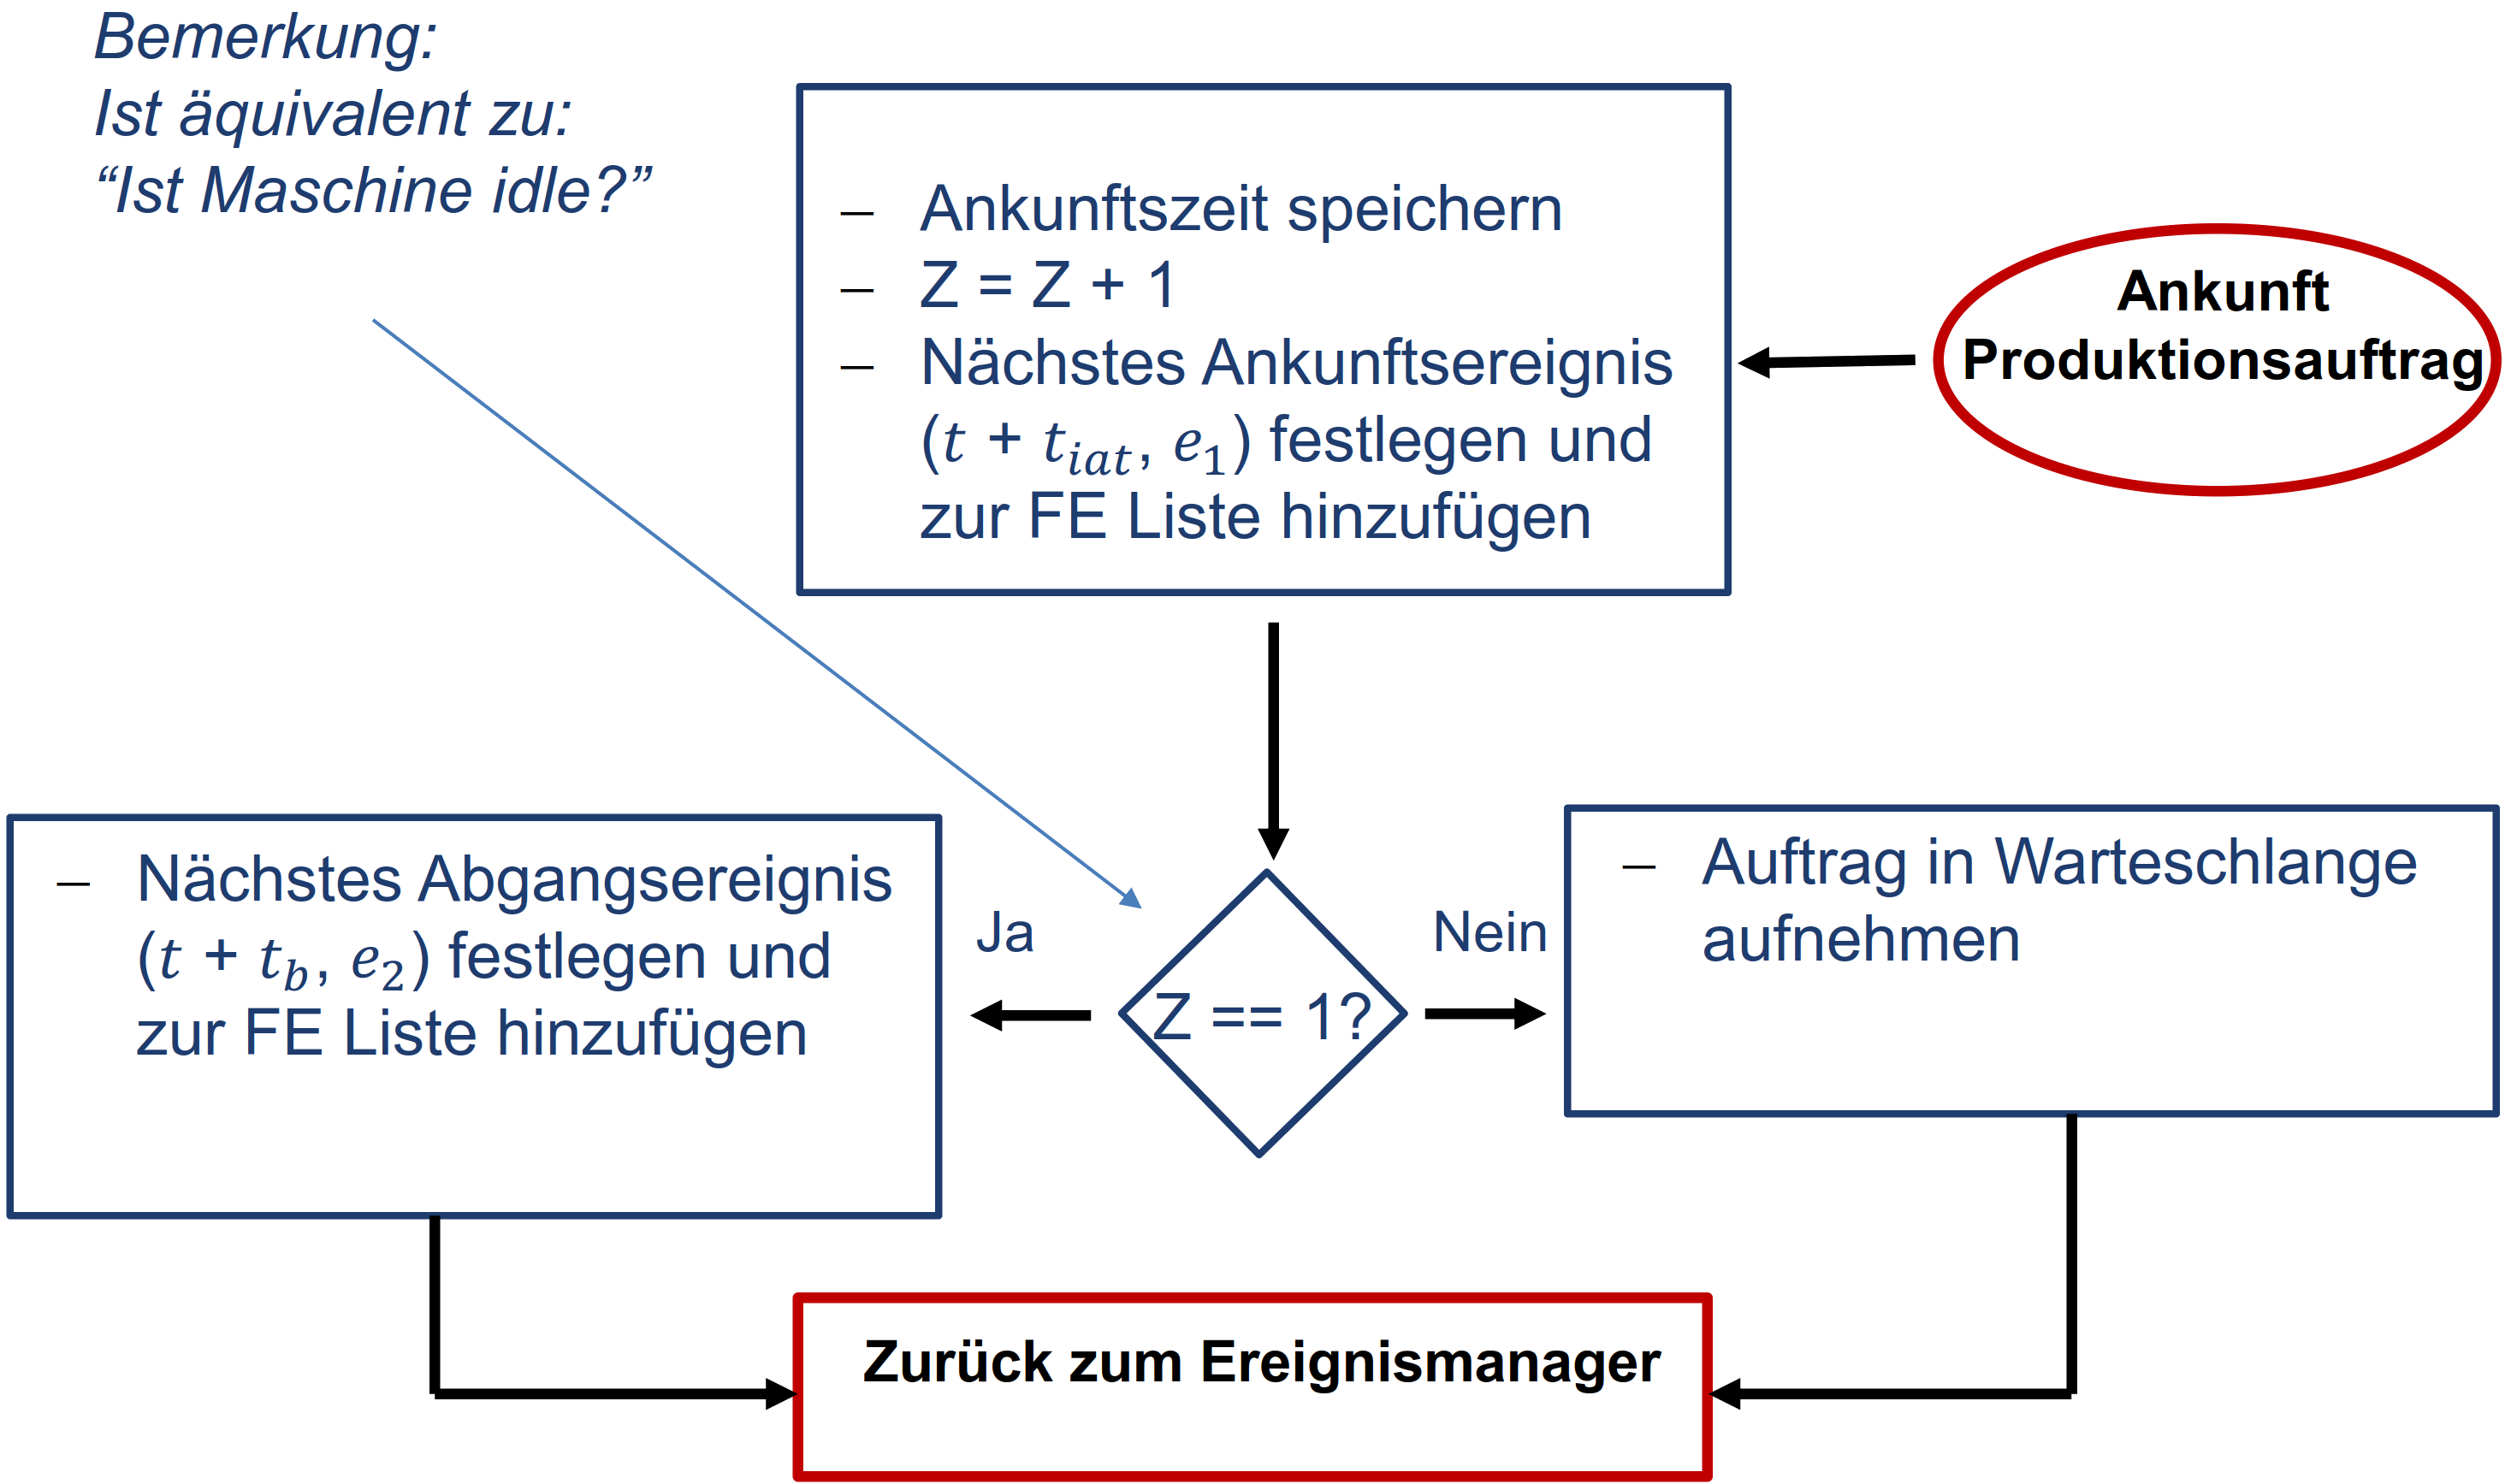
\includegraphics[width=0.5\textwidth]{pictures/ereignisdiagramm1}
		\textbf{Ereignisdiagramm $e_2$:} \\
		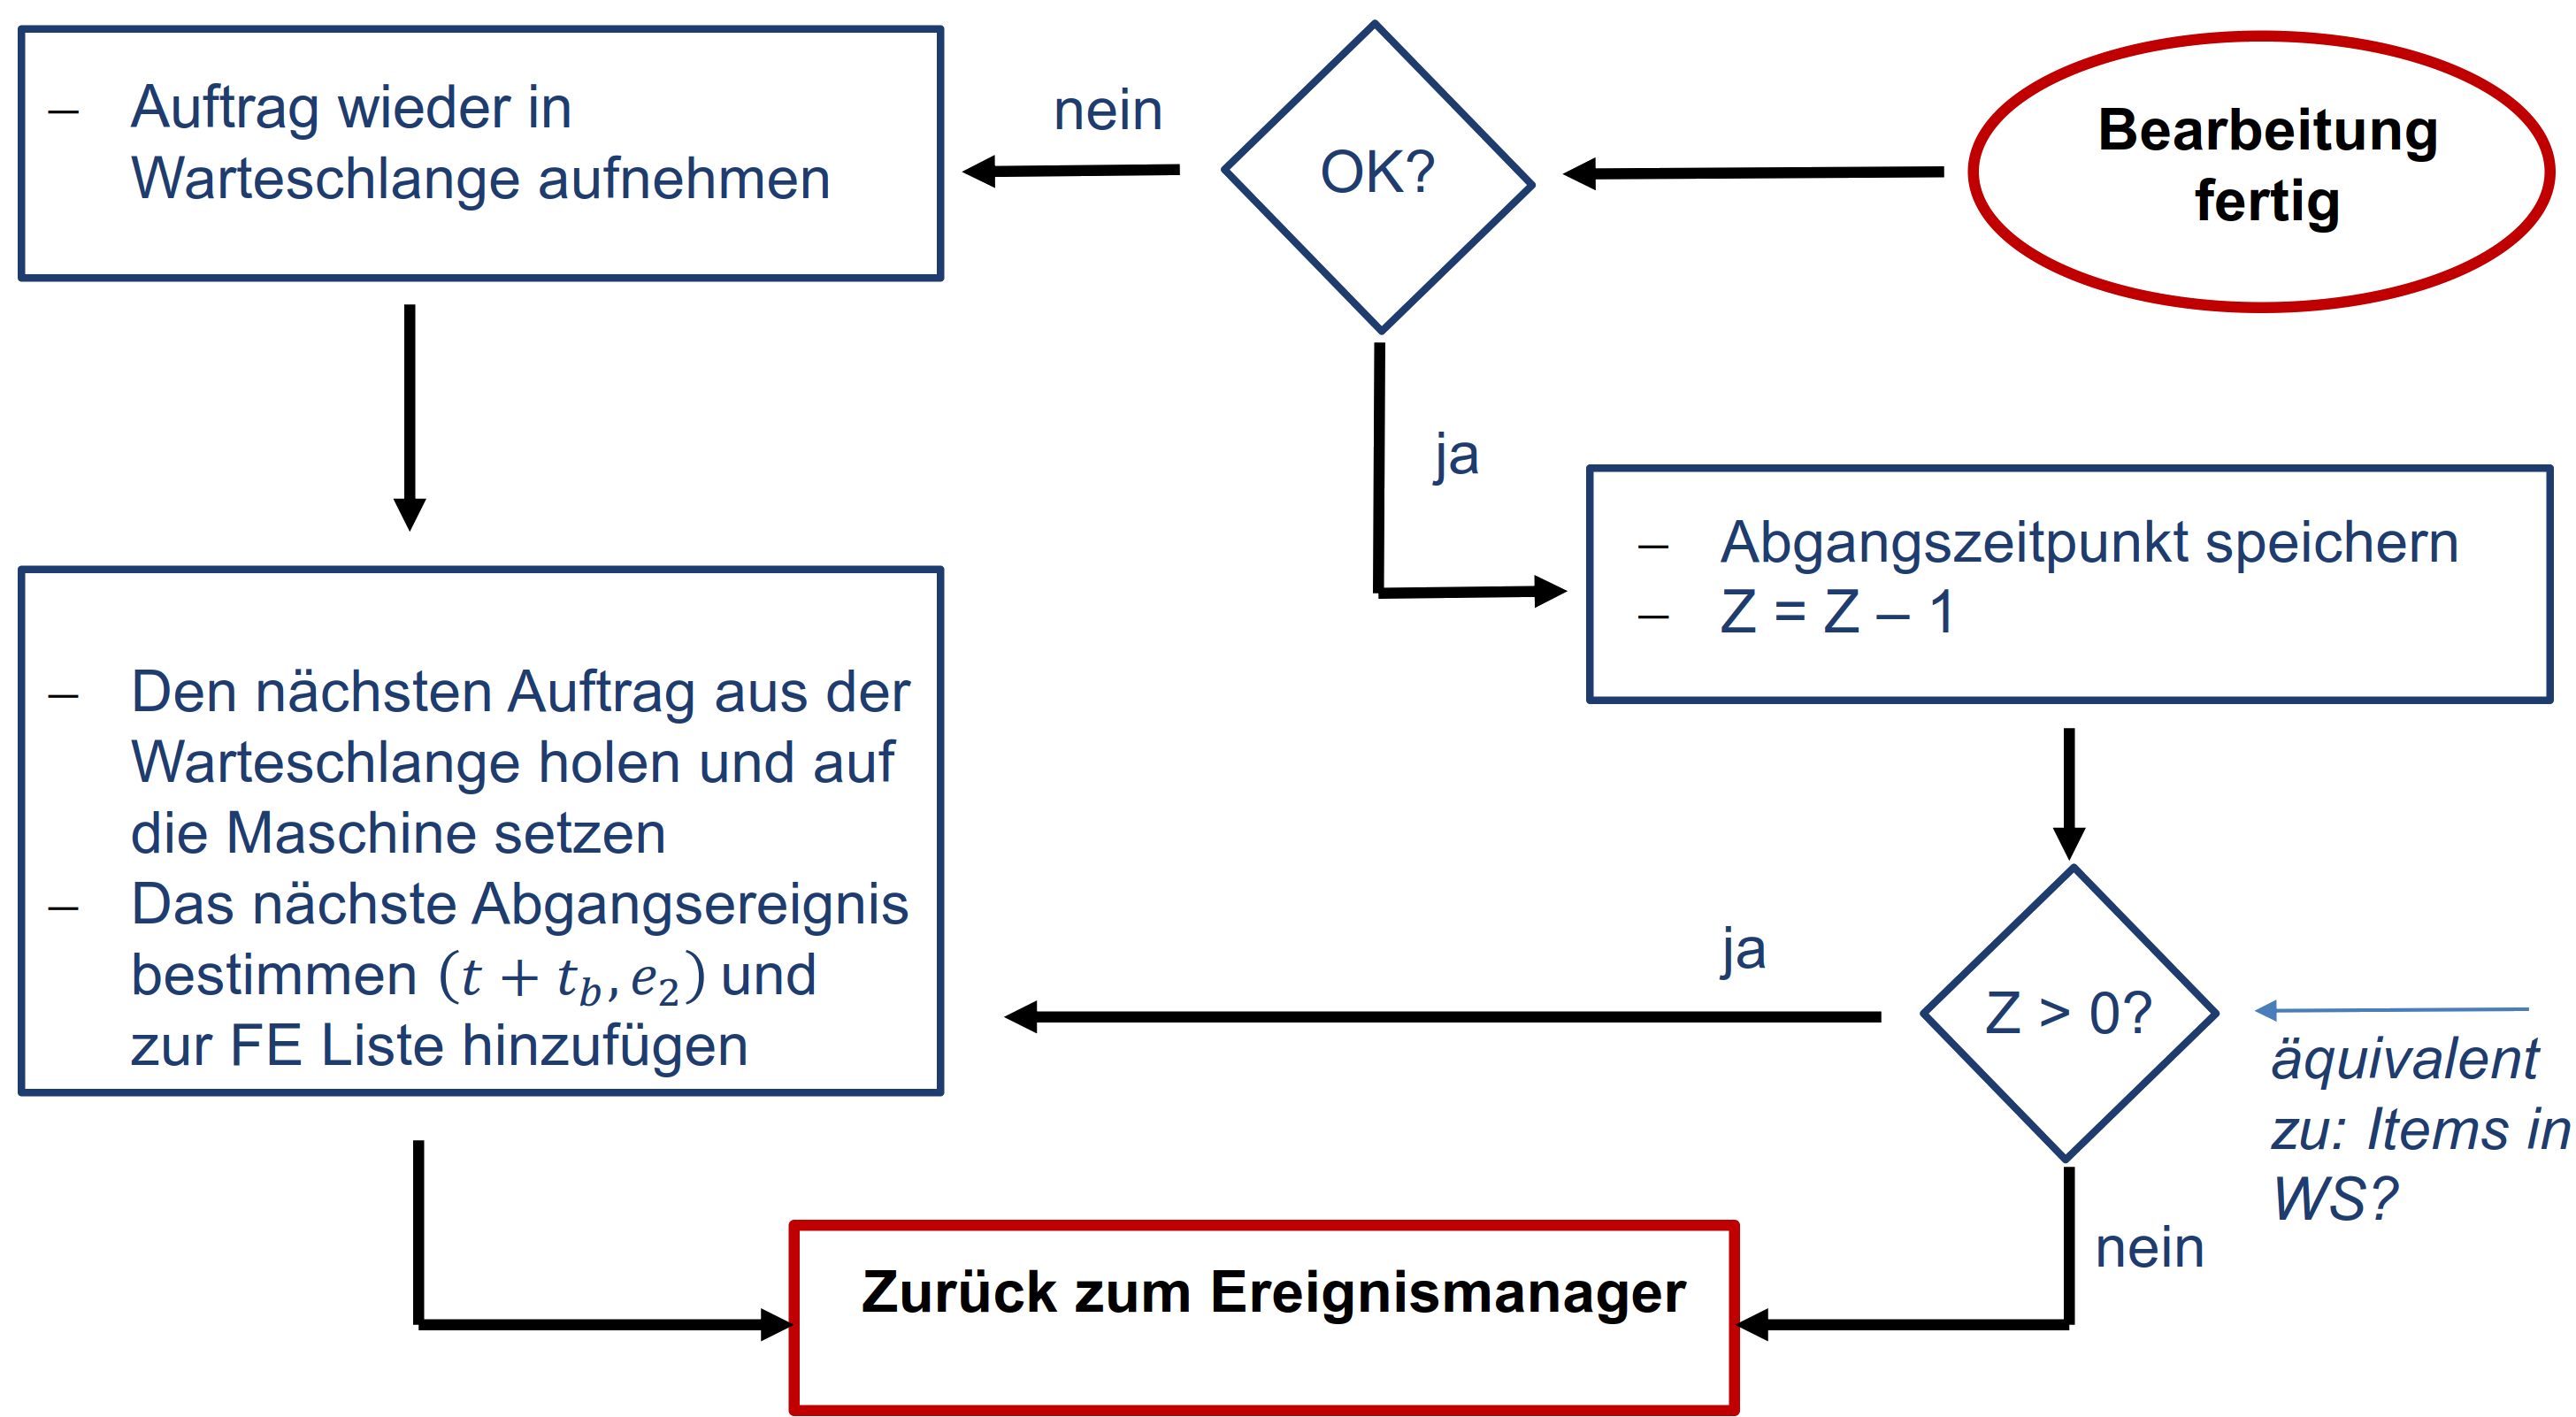
\includegraphics[width=0.5\textwidth]{pictures/ereignisdiagramm2}
	\end{multicols}
\end{example}